\documentclass[12pt]{article}
\usepackage{tikz}

\begin{document}

\begin{center}
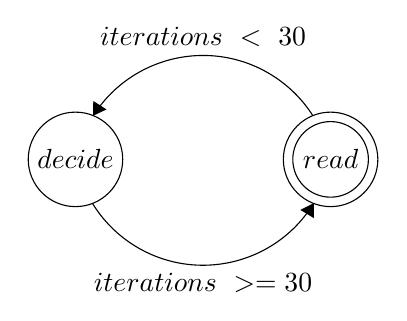
\begin{tikzpicture}[scale=0.2]
\tikzstyle{every node}+=[inner sep=0pt]
\draw [black] (30.8,-30.1) circle (3);
\draw (30.8,-30.1) node {$decide$};
\draw [black] (47,-30.1) circle (3);
\draw (47,-30.1) node {$read$};
\draw [black] (47,-30.1) circle (2.4);
\draw [black] (45.928,-32.884) arc (-31.48101:-148.51899:8.241);
\fill [black] (45.93,-32.88) -- (45.08,-33.31) -- (45.94,-33.83);
\draw (38.9,-37.32) node [below] {$iterations\mbox{ }>=30$};
\draw [black] (31.921,-27.335) arc (147.5502:32.4498:8.271);
\fill [black] (31.92,-27.33) -- (32.77,-26.93) -- (31.93,-26.39);
\draw (38.9,-23) node [above] {$iterations\mbox{ }<\mbox{ }30$};
\end{tikzpicture}
\end{center}

\end{document}

